\documentclass[submit]{aiaa-pretty} %submit, draft, journal options can be used
\usepackage[belowskip=0pt, aboveskip=0pt]{subcaption}
\usepackage{float}
\usepackage{caption}
\usepackage{tcolorbox}
%\setlength{\belowcaptionskip}{-10pt}

%\usepackage{classdiagram}
%\usepackage[T1]{fontenc}

\usepackage{amsmath}
\newenvironment{rcases}
  {\left.\begin{aligned}}
  {\end{aligned}\right\rbrace}
\newenvironment{lcases}
  {\left\lbrace\begin{aligned}}
  {\end{aligned}\right.}

\usepackage{amssymb}
\usepackage{amsfonts}
% * <komahan.cool@gmail.com> 2018-04-24T04:09:52.446Z:
%
% > }
%
% ^.
\usepackage{multirow}
\usepackage{booktabs}
\usepackage{doi}
\usepackage{xcolor}
\usepackage{graphicx,dblfloatfix} 
\usepackage{algorithm}
\usepackage{algpseudocode}
%\usepackage[superscript]{cite}
\usepackage[numbers,compress,sort]{natbib}
%
\usepackage{soul,xcolor}
\setstcolor{blue}

% User defined commands
\newcommand{\ds}{\displaystyle}
\newcommand{\mb}{\mathbf}
\newcommand{\mr}{\mathrm}
\newcommand{\mbs}{\boldsymbol}
\newcommand{\f}{\frac}
\newcommand{\p}{\partial}
\newcommand{\vect}[1]{\vec{\mathbf{#1}}}
\newcommand{\ignore}[1]{}

\renewcommand{\pd}[2]{\displaystyle{\dfrac{\partial #1}{\partial #2}}}
\newcommand{\td}[2]{\dfrac{d #1}{d #2}}
\newcommand{\pdt}[2]{\dfrac{\partial^2 #1}{\partial #2^2}}
\newcommand{\tdt}[2]{\dfrac{d^2 #1}{d #2^2}}
\newcommand{\pdtno}[2]{\dfrac{\partial^2 #1}{\partial #2}}
\newcommand{\pdd}[3]{\dfrac{\partial^2 #1}{\partial #2 \partial #3}}
\newcommand{\pff}[3]{\dfrac{d^2 #1}{d #2 d #3}}

% Redefined commands
\renewcommand\floatpagefraction{.95}
\usepackage{cleveref}
\crefname{subsection}{subsection}{subsections}

%\newcommand{\com}[1]{\textcolor{red}{#1}}
\newcommand{\new}[1]{{\leavevmode\color{black}{#1}}}
\newcommand{\kb}[1]{{\leavevmode\color{blue}{#1}}}
\newcommand{\off}[1]{}
\newcommand{\gjk}[1]{{\leavevmode\color{Red}{#1}}}

\usepackage{cmbright}
%\usepackage{arev}
\renewcommand\familydefault{\sfdefault} 

\usepackage{algorithm}
\usepackage{algpseudocode}

\graphicspath{{talk/}{talk/figures/}{figures/}}

\title{Isogeometric Analysis using NURBS}
\author{Komahan Boopathy  and Siddarth Niranjan\\
  {\normalsize\itshape School of Aerospace Engineering, Georgia Institute of Technology,
    Atlanta, GA, 30332-0150, USA.}\\
} 

\begin{document}
\maketitle
%\abstract{}
\section{Introduction}

Figure~\ref{fig:iga-demo} 
\begin{figure}[h] 
  \centering
  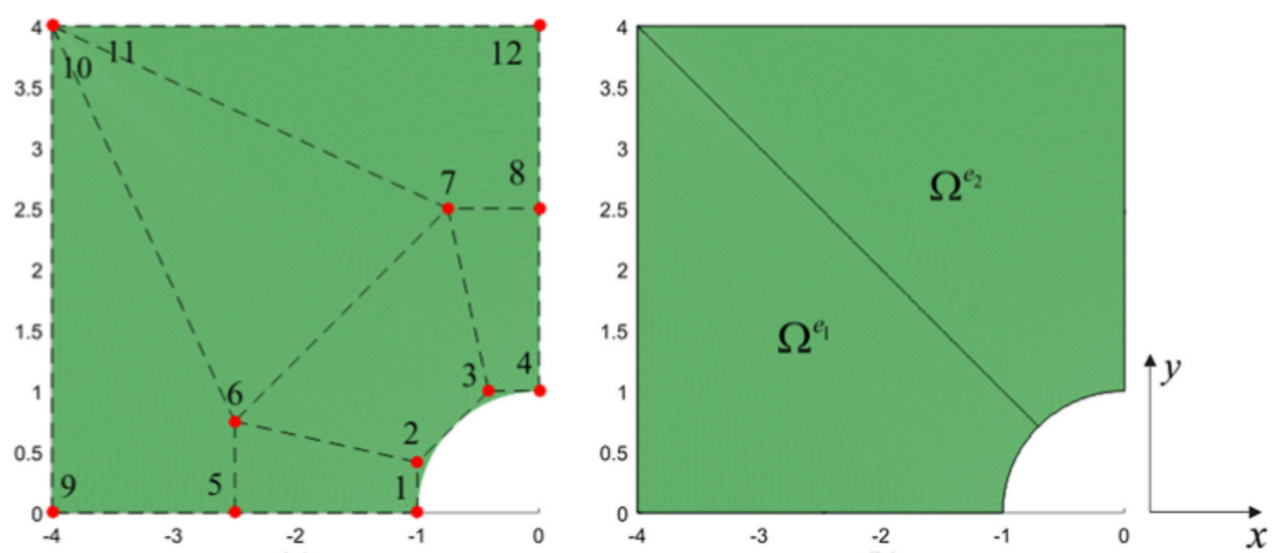
\includegraphics[width=1.0\linewidth]{iga-demo.pdf}
  \caption{\emph{}}
  \label{fig:iga-demo}
\end{figure}

\bibliographystyle{myabbrvnat}
\bibliography{references}

\end{document}

\section{Introduction and Motivation}

% Philosophy is a whole body of inter-related principles.
% A principle, in this context, is a rule of thinking. 
% Philosophy is the study of all rules of thinking.

%attributes and behavior

The interplay of \emph{geometry}, \emph{calculus} and \emph{algebra}
is at the heart of contemporary scientific and engineering problems of
interest, and running across these mathematical subjects is the
science of \emph{computing}. Let us first explore how these subjects
work together in solving problems of interest, and in shaping the
motivation for this project.
%\subsection{Solution Process of PDEs}
Geometrical concepts attempt to describe the shape and size of
physical objects (e.g. spheres, cubical containers, airplanes and
human body) in terms of intuitive quantities such as \emph{curvature},
\emph{lengths}, \emph{areas} and \emph{volumes}.
% \footcite{There are more advanced concepts as well but these are essential.}
We can \textbf{associate} any tensorial
%\footnote{Tensors
%  give a sense of direction to the fields that we consider. For
%  example, scalar fields do not require a sense of direction, where as
%  first order tensors (the vector) and second order tensors (the
%  dyadic) require one and two directions respectively. This
%  generalizes to higher-order tensors as well when more and more
%  senses of directions are required to fully characterize the field.}
field of interest $\phi$ with these geometrical \textbf{object}
based on our needs (e.g. temperature, velocity, pressure, wing deflection,
strain on an airplane).  For computational purposes we first tend to discretize the
geometry object into a discretized/parametrized geometry, termed as a
mesh, which is simply a \emph{set}
%\footnote{a type of collection where uniqueness is required} of
nodes with an associated \emph{topology}. Then, each node in the
geometry has the set of fields $\phi$. Because, the field that we
associate to each node are assumed to \emph{vary} as a
\textbf{function} of geometric \textbf{parameters}
%\footnote{ In many cases, parameters other than space and time come
%  into play such as material properties (e.g. viscosity of fluid,
%  rigidity modulus of a bar geometry in torsion), but the same
%  machinery of calculus applies invariably, and therfore shall limit
%  our discussion to these intuitive geometrical parameters for better
%  exposition of concepts and issues.  } (e.g. spatial locations,
%time), 
we introduce the term \emph{field variables}, also referred to
as \emph{state variables}. These fields can be called as geometrical
fields or space time fields, or simply functions of the 4-dimensional
space-time geometry. The \textbf{abstraction} of \emph{space-time
  fields} (e.g. $\phi({x,t})$) as \emph{parametric fields
  $\phi({\xi})$} can be made if one works with a general set of
parameters. Calculus, the study of change, by means of ordinary and/or
partial differential equations attempts to model and describe the
\emph{change in field with its parameters} as accurately as
possible. A branch of calculus, namely \emph{the calculus of
  variations} provides a unified framework for obtaining these
governing differential equations for change in fields, when certain
requirements are met~\cite{Lanczos2015}. The linear and non-linear algebra
framework (e.g. Newton's method, GMRES etc) aids in solving
\emph{algebraic} linear or non-linear systems of equations and provide
us with the solution of field variables and their derivatives. The
\textbf{casting} of differential equations into algebraic form amenable
for the algebraic machinery is addressed by spatial-discretization
techniques such as finite element method, finite difference method,
finite volume method, spectral method and boundary element methods.
While the roles of geometry, calculus and algebra are apparent from
the above discussion, the role of computing is rather obscure at this
level of presentation. At this juncture, it is noted that the words in
boldface in the above discussion, pertains to ideas/concepts in
computer programming. Thus, a careful description of concepts by
engineers and scientists in describing the problems greatly helps a
computer programmer in forming numerical data structures and
implementing solution principles as algorithms.
The process of solving the PDEs, in computer science terminology
can be called casting to lower-dimensional objects. If PDEs are of the
highest abstraction, then they are cast into ODEs (using FVM/FEM/FDM), which
are in-turn cast into Nonlinear systems of equations, that are then
linearized and handed over to the very mature machinery of linear
algebra. 
%Formalisms are mathematical abstractions that can be applied to a wide
%range of physical scenarios.
%By applying the abstract mathematical operations on
%different functionals, one can obtain parametric sensitivities of quantites and statistics
%(mean and standard deriviation) of quantities in an efficient manner.
%\subsection{General PDE Solution}
A general philosophy followed in solving partial differential equations are as follows:
\begin{enumerate}
\item formulation of governing partial differential equations (PDEs)
\item spatial discretization of PDEs to cast them as ordinary
  differential equations (ODEs)
\item Casting of ODEs to nonlinear and linear algebraic system of equations
\end{enumerate}
This is illustrated in Figure~\ref{fig:solution_flow}. The entire solution framework requires a lot of guiding principles,
however, only a few are illustrated in the schematic.
\begin{figure}[H]
  \centering 
  \includegraphics[width=0.25\linewidth]{solution-flow.pdf}
  \caption{An illustration of typical solution process adopted for
    nonlinear partial differential equations.}
  \label{fig:solution_flow}
\end{figure}
 The importance of unifying existing numerical schemes under a common
 framework is felt undermined and such efforts need to arise in order
 to be able to solve these equations better in a flexible manner. To
 elaborate this point a little further, a following demonstration is
 considered.  We today have canned functions to compute matrix
 inverses, factorization, linear transformations such as Fourier and
 Laplace transform and so on. The linear algebra machinery is very
 mature that one can expect to solve a linear system using a variety
 of available method like a black box with zero intrusiveness with the
 solution process itself. If one provides a matrix $A$ and the right
 hand side $b$, the solution $x$ can be obtained in a robust
 manner. Similarly if one uses an iterative method, and providing
 inner products and Jacobian-vector product is solely enough to solve
 the linear system iteratively. For solving nonlinear problems, we
 linearize the problem and use the robust linear algebra machinery to
 solve the nonlinear system.  For ordinary differential equations
 (linear and nonlinear), we have time marching methods and
 implementations to use to solve them in time.  When it comes to
 partial differential equations, such general packages are
 non-existent.  As the physics community is looking for unifying
 existing governing equations, it is not irrelevant to develop new
 solution procedures and bring existing ones under a common unifying
 solution framework. The utility of such an effort is enormous.
 However, efforts have been made and under continued development to
 bring the solution under a common framework such as
 FENICS~\cite{AlnaesBlechta2015a}, DOLFIN~\cite{LoggWellsEtAl2012a},
 UFC~\cite{AlnaesLoggEtAl2012a} and others.

\subsection*{Scope of this Work}

In this project, a part of this voluminous effort is considered -- to
develop a minimal solution framework that can solve simple partial
differential equations with minimal set of requirements like forming
vectors and matrix-vector products using finite volume method as the
discretization approach.
This work involves the implementation of mesh processing capabilities,
linear and nonlinear solvers for algebraic equations and time marching
methods for ODEs. 
The software architecture involved in solving PDEs is discussed.
Interesting findings and implementation issues are identified and
discussed in relevant sections. 
Finally demonstrations are shown on steady heat equation.


%solution approches amd The scope of this project is to solve simple
%partial differential equations using finite volume method a Formalisms
%are mathematical abstractions that can be applied to a wide range of
%physical scenarios.

\section{Method: Data structures and Algorithms}

A general process flow in solving PDEs on which the framework is built
is shown in Figure~\ref{fig:solution_flow2}.
\begin{figure}[h!]
  \centering 
  \includegraphics[width=0.6\linewidth]{process-flow.pdf}
  \caption{Abstract process designed for solving PDEs.}
  \label{fig:solution_flow2}
\end{figure}
The data structures and algorithms pertaining to this process flow are
discussed in the remainder of this section. Since we intend to design
the framework for general PDEs, it suffices to represent them in
abstract mathematical implicit form as:
\begin{equation}
  \mathbf{R}(\mathbf{U}, \mathbf{\dot{U}},\mathbf{ U'}; x, t) = 0.
\end{equation}
Although, the motivations suggest the abstraction of space time
parameters $\mathbf{x}$ and $t$, and others, as an array of general
parameters $\xi$, we stick to the basic form for intuitive
understanding of the process and development of computational
machinery.

\subsection{Mesh Data structure}
The goal of meshing is to discretize the spatial domain $\Omega$ into
simplex geometry entities listed in
Table~\ref{tab:basic_simplex_entries} and their generalizations.
The reason one works with simplex entities is that the geometry is
easier to handle compared to curved geometries.
At the end of meshing process, any complex domain is given an
equivalent representation in terms of a collection of simplex
entities. 
\begin{table}
  \caption{Basic simplex entities and mesh terminology.}
  \centering \scalebox{1.0}{
    \begin{tabular}{c|cccc}
      \toprule
      Dimension & Basic Simplex & Mesh Terminology \\
      \midrule
      0 & point & vertex \\
      1 & line & edge \\
      2 & surface & face \\
      3 & volume & cell \\
      \bottomrule
    \end{tabular}
  }
  \label{tab:basic_simplex_entries}
\end{table}
\begin{figure}[h]
  \centering
  \begin{subfigure}{0.3\textwidth}
    \includegraphics[width=\linewidth]{mesh-20.eps}
  \end{subfigure}
  \begin{subfigure}{0.46\textwidth}
    \includegraphics[width=\linewidth]{fvm-terminology.pdf} 
  \end{subfigure}
  \caption{An example of a two-dimensional unstructured meshes with
    triangular cells (left) and two cells sharing a face (right).}
  \label{fig:geometry-grid}
\end{figure}
 An unstructured (numbered) mesh is one that does not have a regular
 ordering of cells. The numbering pattern is arbitrary and therefore
 they need to be stored additionally. In general, the iteration
 fashion in unstructured mesh is contingent with the numbering of
 cells, \emph{i.e.,} we may not follow left to right/ bottom to top
 way of traversing the domain when looping as in the case of
 rectangular mesh.  Another striking characteristic of unstructured
 mesh is that it does not always contain rectangular/Cartesian
 entries.  We consider only two-dimensional geometries in this work,
 therefore, \emph{cells} refer to \emph{triangles/quadrilateral} and
 \emph{faces} refer to the edges of triangles/quadrilaterals.
  \begin{figure}[h]
   \centering
   \includegraphics[width=0.25\textwidth]{mesh-type.pdf}
   \caption{Class diagram of mesh data structure for handling
    unstructured geometries.}
   \label{fig:mesh-type}
\end{figure}
A computational mesh object has the following information encapsulated:
\begin{itemize}
\item geometry (areas, lengths, volumes, centers)
\item topology (connectivities), 
\item weights for interpolation, counts of vertices, faces and cells 
\item tagging of elements for associating different parts of domain with relevant
  physics equations (geometry-physics connectivity)
\item interpolation weights
\end{itemize}
A mesh data structure is implemented encapsulates basic and derived
topology information, along with geometric quantities related to the
elements in mesh. This is shown in the class diagram in
Figure~\ref{fig:mesh-type}.  It contains basis simplex entities like
cells, faces and vertices. The topological connectivities between
higher and lower dimensional entities and their reverse mapping are
also stored.  The geometrical quantities (areas, volumes, lengths,
normals, tangents etc) are computed once and stored for subsequent use
in the mesh object. 
This information is vital for the formation of
linear system with the application of finite volume method.  The mesh
object also tags the cells and faces. This allows the application of
boundary conditions on $\partial \Omega$ and governing equations on
$\Omega$.  In finite volume method, distance weighed interpolations
are used for computing face center values from cell center values and
also vertex values from cell values. These weights are computed once
and stored for repeated use.
In summary, any information about geometry and mesh needed by the solver
is obtained only from the mesh object.

\subsubsection*{Creation of Mesh Object}

The mesh files are created using an open-source program
GMSH~\cite{Geuzaine2009}. GMSH is a finite element mesh generation
program. It provides only a part of the basic topological
connectivities that are necessary in a finite volume method. For
example, the edges of the triangles/quadrilateral objects are not
exported directly from the meshing program. Therefore, the faces are
formed as an ordered pair of nodes internally in the framework's
\texttt{Mesh} class. This currently, is a bottleneck and an expensive
operation for large mesh sizes -- it turns out that the solution is
faster than the identification of faces in the geometry!  The current
work flow is that the mesh is loaded into memory most of the basic
topology information (except face numbers) are available readily in
the mesh file. The derived topology information (inverse
connectivities), geometrical quantities and weights are then computed
using the \texttt{Mesh} class.

\subsection{Integration Interface}
The time integration interface is design to solve problems of the
abstract form shown in Figure~\ref{fig:solution_flow2}. Implicit
methods require the solution of the linearized-nonlinear-system of the
form
  \begin{equation}
    \label{eqn:linearized} \left[ {\alpha} \pd{\mathbf{R}}{\dot{\mathbf{Q}}} +
    \pd{\mathbf{R}}{{\mathbf{Q}}} \right]_{m \times m} \left\{\mathbf{Q}\right\}_{m \times
    1} = - \left\{ \mathbf{R} \right\}_{m \times 1} 
    \end{equation}
  where $\pd{\mathbf{R}}{\dot{\mathbf{Q}}}= {\cal{I}}$,
  $\alpha=\pd{\dot{\mathbf{Q}}^{n}}{\mathbf{Q}^n}$, and $m$ is the
  total number of state variables which is equal to the number of
  interior nodes in mesh. Table~\ref{tab:integation_schemes} lists the
  integration schemes that implement the interface of parent
  integrator class and their properties.
  \begin{table}
    \centering
    \caption{Integration schemes, solution method and order of accuracy.}
    \label{tab:integation_schemes}
    \begin{tabular}{lcc}
      \hline
      Scheme         & Order of accuracy & Solution method \\
      \hline
      Backward Difference Formulas    & 1-6 & implicit multistep  \\
      Adams Bashforth Moulton         & 1-6 & implicit multistep  \\
      Diagonally implicit Runge--Kutta & 2-4 & implicit multistage \\
      \hline
    \end{tabular}
  \end{table}

\subsection{Nonlinear Solver Interface}
The \texttt{NonLinearSolverInterface} defines the interface necessary
for extending \texttt{NonLinearSolver} classes to implement. An
implementation of Newton's method is provided by extending this
interface. The algorithm is shown below.
\begin{algorithm}[H]
  \caption{Newton method for the solution of nonlinear system.}
  \label{alg:newton-krylov}  
  \begin{algorithmic}[1]
    \Require $\epsilon$ \Comment{solution tolerance}
    \Require nmax \Comment{maximum number of allowed iterations}
    \Require $\mathbf{Q}_0, \mathbf{\dot{Q}}_0$ \Comment{solution guess}
    \For {n = 1, nmax} 
    \State $\mathbf{R}_n \leftarrow$ evaluate\_residual($\mathbf{Q}_n$,$\mathbf{\dot{Q}}_n$)\Comment{Governing Equation}
    \If {$||\mathbf{R}_n||_2 < \epsilon$} \Comment{check convergence}
    \State \Return  $\mathbf{Q}_n, \mathbf{\dot{Q}}_n$
    \EndIf
    \State LinearSolve $\left[ \pd{\mathbf{R}}{\mathbf{\dot{Q}}} + h \alpha  \pd{\mathbf{R}}{\mathbf{\dot{Q}}} \right] \mathbf{\Delta \dot{Q}} = -R$ \Comment{Gauss/Conjugate Gradient}
    \State $ \mathbf{Q}_{n+1} \leftarrow \mathbf{Q}_n + \mathbf{\Delta Q}_n$ \Comment{update state solution}
    \State $\mathbf{\dot{Q}}_{n+1} \leftarrow \mathbf{\dot{Q}}_n + h \alpha\mathbf{\Delta \dot{Q}}_n$ \Comment{update state derivative solution}
    \EndFor
  \end{algorithmic}
\end{algorithm}
The nonlinear solver is used the by time integrators at each time step.

\subsection{Linear Solver Interface}
The \texttt{LinearSolverInterface} defines the interface necessary for
extending LinearSolver classes to implement.
Classes that implement this interface only provide information on how
one step of iteration is carried out. The parent interface is
responsible for the coordinates the linear solution process $R = b-Ax
\le \epsilon$, by calling the provided iteration behavior repeatedly
until convergence.  The inheritance hierarchy is shown
in Figure~\ref{fig:linear_solver_hierarchy}.
\begin{figure}[H]
  \centering 
  \includegraphics[width=0.25\linewidth]{linear-solver-framework.pdf}
  \caption{Inheritance hierarchy of linear solver framework.}
  \label{fig:linear_solver_hierarchy}
\end{figure}
The classical iterations or Krylov methods extending the interface
will only have to provide implementation to \texttt{iterate()}
function.

\subsubsection{Krylov-Subspace Methods}

Methods such as Conjugate-Gradient, GMRES, CGNE, CGNR, Bi-CG fall
under this category of methods that work on the \textbf{principle of
  orthogonalization} starting from an arbitrary vector. This method
only requires the evaluation of residual at each iteration and
full-matrix-vector products during each iteration. This information is
readily provided by the \texttt{Assembler} object. The following
algorithm outlines the Conjugate-Gradient Solver implemented within
the \texttt{LinearSolver} framework.

\begin{algorithm}
  \caption{Conjugate-Gradient algorithm implemented within the
    framework.}
  \label{alg:conjugate-gradient}  
  \begin{algorithmic}[1]
    \Require $\epsilon$ \Comment{solution tolerance}
    \Require $\mathbf{x}_0$ \Comment{solution guess}
    \State $\mathbf{b}_0 \leftarrow$ evaluate\_residual(source) \Comment{evaluate source term}
    \State $\mathbf{r}_0 \leftarrow$ evaluate\_residual() \Comment{evaluate full residual}
    \State $\tau = |r_0|_2/|b_0|_2$ \Comment{update stopping criteria}
    \While {$\tau > \epsilon$}
    \If {first iteration} \Comment{check convergence}
    \State p = r \Comment{steepest descent direction}
    \State $\rho_2 \leftarrow |r_0|^2$
    \ElsIf
    \State $p = r + \frac{\rho_2}{\rho_1} p$ \Comment{conjugate direction}
    \EndIf   
    \State $\mathbf{w} \leftarrow$ Jacobian\_vector\_product(p) \Comment{Compute solution update}
    \State $ \alpha \leftarrow \rho_2/\mathbf{p}^T\mathbf{w}$ \Comment{compute step size for update}
    \State $ \mathbf{x} \leftarrow \mathbf{x} +\alpha \mathbf{p}$ \Comment{update new solution}
    \State $ \mathbf{r} \leftarrow \mathbf{r} -\alpha \mathbf{w}$ \Comment{update new residual}
    \State $\tau = |r|_2/|b|_2$ \Comment{update stopping criteria}
    \State $\rho_1 \leftarrow \rho_2$
    \State $\rho_2 \leftarrow |r|^2$    
    \EndWhile
  \end{algorithmic}
\end{algorithm}
It is known that conjugate gradient method works only for symmetric
linear systems. In order to handle non-symmetric cases, a minor
variant of CG, namely the CGNE method is implemented. This method
solves $A^TAx=A^TB$. Therefore, if the linear system is determined to
be non-symmetric, then each vector resulting in the above algorithm is
multiplied by a transpose-jacobian-vector product.

\subsubsection{Classical Methods}

The classical iteration methods work on the \textbf{principle of
  splitting} of matrix $A$ into different parts and moving the
difficult part over to the right hand side and iterate. The
implementation of classical methods is more involved than
Krylov-Subspace methods, in terms of matrix assembly operations. The
classical iterations also can be implemented in matrix-vector-assembly
framework, however, they only require parts of matrix (diagonal, lower
and upper triangle matrices) unlike Krylov-methods that use
full-matrix-vector product. This gives rise to additional
complications during Jacobian-vector products.
The full Jacobian matrix $A$ is assembled/split such as $A=D+L+U$ and
classical iteration formulae are applied until the norm of the
residual $R^k=\Delta x^k = b-Ax^k$ falls below a tolerance of
$10^{-14}$.
%\paragraph{\textbf{Gauss Jacobi Iteration}}
In Gauss--Jacobi method, the linear system is solved as
\begin{equation}
  D x^{k+1} = b - L x^{k} -U x^{k}.
\end{equation}
%\paragraph{\textbf{Gauss Seidel Iteration}}
In Gauss--Seidel method, the linear system is solved such that
\begin{equation}
  (L + D) x^{k+1} = b - U x^{k}.
\end{equation}
The lower triangular system is solve iteratively using a Jacobi like
inner iteration.
%\paragraph{\textbf{Successive Over Relaxation}}
In {Successive Over Relaxation method}, the matrix is split with an
assigned weight $\Omega$
\begin{equation}
   (D + \Omega L)x^{k+1} = \Omega (b-Ux^k) + (1-\Omega) D x^k
\end{equation}
For the case of structured mesh, it is intuitive on which entries go
into lower triangular part and which entries go into the upper
triangular part. However, for unstructured mesh this is not as
intuitively straightforward -- but it turns out that the solution is
much simpler than it appears! The following algorithm illustrates the
simplicity of the solution to this issue.
\begin{algorithm}[H]
  \caption{Matrix Filtering Algorithm for Unstructured Meshes during finite volume assembly.}
  \label{alg:matrix-filter}  
  \begin{algorithmic}[1]
    \For {icell = 1, ncells} \Comment{loop cells}
    \State Ax(icell) = 0 \Comment{Initialize Matrix Vector product}
    \For {iface = 1, num\_cell\_faces} \Comment{loop cell faces}
    \State ncell = GetNeighbouringCell(iface, icell)\Comment{Neighbor to this cell along this face}
    \If {ncell $>$ icell} \Comment{Upper Diagonal Contribution}
    \State \texttt{Ax(icell) = Ax(icell) + farea*(x(ncell))/fdelta}
    \ElsIf {ncell $<$ icell} \Comment{Lower Diagonal Contribution}
    \State \texttt{Ax(icell) = Ax(icell) + farea*(x(ncell))/fdelta}
    \ElsIf {ncell $=$ icell} \Comment{Diagonal Contribution}
    \State \texttt{Ax(icell) = Ax(icell) + farea*(-x(icell))/fdelta}
    \State \texttt{Ax(icell) = Ax(icell) + farea*(-x(ncell))/fdelta}
    \EndIf
    \EndFor
    \EndFor
  \end{algorithmic}
\end{algorithm}
Thus, classical iteration equations are implemented using ``masked''
matrix-vector products. The ``masks'' are supplied as input to the
\texttt{Assembler} object which coordinates the mesh and physics
internally to return the required matrix-vector products.

\subsection{Assembler Interface}

All the solution-level interfaces for solving linear and nonlinear
system and the algorithms discussed need, residual assembly (or parts
of it) and Jacobian-vector products (or parts of it). The
\texttt{Assembler} class is designed precisely to abstract the supply
of these two essential ingredients. The schematic of the
\texttt{Assembler} object is shown in Figure~\ref{fig:assembler_obj}. 
\begin{figure}[H]
  \centering 
  \includegraphics[width=0.35\linewidth]{assembler-type.pdf}
  \caption{The \texttt{Assembler} data type, its attributes and functions.}
  \label{fig:assembler_obj}
\end{figure}
 In a nutshell, the \texttt{Assembler} object coordinates the
 \texttt{Mesh}, \texttt{Physics}, \texttt{Discretization} in obtaining
 the information necessary for solution. In this work only finite
 volume method is used for discretization and therefore it is limited
 to FVM. However, if we consider to implement other techniques like
 finite element method the discretization can be abstracted out of the
 \texttt{Assembler} and supplied as an user input. This, in principle,
 is easier, but implementation can be extremely hard : currently,
 there is no state of the art tool/framework that allows one to swap
 out discretization techniques as an user input. Such a feature will
 give one enormous flexibility in solving classes of PDEs
 efficiently. The abstraction of discretization holds the key for this
 advancement.  Another point to note is that, for non-symmetric
 matrices use of CG method requires transpose-jacobian-vector
 products.  We can use the same Matrix Filter
 Algorithm~\ref{alg:matrix-filter} by simply swapping the definition
   of lower diagonal and upper diagonal contributions!

\section{Computational Analysis}

The above framework is applied to solve a 2D problem with nontrivial
geometry and an 1D advection diffusion problem.


\subsection{2D Steady State Heat}

\subsubsection{Governing Equations and Boundary Conditions}
We consider the solution the two dimensional steady heat equation on
unstructured meshes using the discussed framework. The governing
equation is
$\nabla . \nabla T(x,y) = 0.$
We consider different Dirichlet boundary conditions as shown in 
Table~\ref{tab:model_problem}.
\begin{table}[H]
  \centering
  \caption{Boundary conditions for model problem.}
  \label{tab:model_problem}
  \begin{tabular}{l|cccc}
    \toprule
    case & bottom & right & top & left \\
    \midrule
    1 & 0 & 0 & 0 & 1 \\
    2 & 0 & 1 & 0 & 0 \\
    \bottomrule
  \end{tabular}
\end{table}
In the first case, the left wall is maintained at a higher
temperature than the other three walls. In the second case, the bottom
wall is maintained at a higher temperature than the other three walls.
The tagging of faces and cells in the \texttt{Mesh} objects allows us
to apply the boundary conditions on the specific entities of interest.

\subsubsection{Geometries and Mesh}

We study the steady state heat distribution in the square domain when
non-trivial geometrical entities are present. For this we pick the
case of a rectangular domain with a central cylinder and airfoil and
solve the heat equation using finite volume method. The Mesh handler
class is general that it can handle heterogeneous mesh types. The mesh
can contain quadrilateral and triangular elements. In order to
demonstrate this functionality, we generated two sets of meshes:
triangular and rectangular for one of the geometries. These meshes are
created using an open-source program GMSH~\cite{Geuzaine2009}. 


\subsubsection{Temperature Distributions}
Figures~\ref{fig:temp_tria} and ~\ref{fig:temp_tria2} show the
temperature distributions obtained using triangular mesh elements for
both boundary conditions. It can be seen that the solution makes
intuitive sense as to a smooth distribution of temperature from hot
wall to cold wall. Interesting patterns are formed around the
geometric obstacles placed in the rectangular domain. The distribution
is horizontally symmetric in Figure~\ref{fig:temp_tria}, as the
airfoil is at zero pitch angle.
\begin{figure}[H]
  \centering
  \begin{subfigure}{0.49\linewidth}
    \includegraphics[width=\textwidth,trim={4pt 4pt 4pt 4pt},clip]{cylinder-steady-temp-1.png}
    \caption{cylinder}
  \end{subfigure}
  \begin{subfigure}{0.49\linewidth}
    \includegraphics[width=\textwidth,trim={4pt 4pt 4pt 4pt},clip]{airfoil-steady-temp-1.png}
    \caption{airfoil}
  \end{subfigure}
  \caption{Temperature distribution obtained using triangular mesh for boundary conditions set 1.}
  \label{fig:temp_tria}
\end{figure}
However for the second case in Figure~\ref{fig:temp_tria2}, the
symmetry is lost due to the nature of the geometry and boundary
condition (see airfoil).
\begin{figure}[H]
  \centering
  \begin{subfigure}{0.49\linewidth}
    \includegraphics[width=\textwidth,trim={4pt 4pt 4pt 4pt},clip]{cylinder-steady-temp-2-1.png}
    \caption{cylinder}
  \end{subfigure}
  \begin{subfigure}{0.49\linewidth}
    \includegraphics[width=\textwidth,trim={4pt 4pt 4pt 4pt},clip]{airfoil-steady-temp-2-1.png}
    \caption{airfoil}
  \end{subfigure}
  \caption{Temperature distribution obtained using triangular mesh for boundary conditions set 2.}
  \label{fig:temp_tria2}
\end{figure}
The mesh handler can process a mesh with quadrilateral cells which is
demonstrated using Figure~\ref{fig:temp_quad}.
\begin{figure}[H]
  \centering
  \begin{subfigure}{0.49\linewidth}
    \includegraphics[width=\textwidth,trim={4pt 4pt 4pt 4pt},clip]{airfoil-quad-1-1.png}
    \caption{BC 1}
  \end{subfigure}
  \begin{subfigure}{0.49\linewidth}
    \includegraphics[width=\textwidth,trim={4pt 4pt 4pt 4pt},clip]{airfoil-quad-2-1.png}
    \caption{BC 2}
  \end{subfigure}
  \caption{Temperature distribution obtained using quadrilateral mesh.}
  \label{fig:temp_quad}
\end{figure}

Note that this framework was used to solve the homework 2 problem for
the same physics but on a simpler geometry. The rate of convergence
has been demonstrated to be 1.4 (due to first order implementation of
boundary conditions). 

\subsubsection{Analysis Setup}
Here, the typical setup of analysis is described. For this
demonstration case, four linear solvers are used to solve the model
problem : Jacobi, Seidel, CG and SOR. The basic steps involved in the
framework are described below.
\begin{itemize}
\item The First, the mesh object is created using the
  \texttt{GmshLoader} class.
\item The mesh object is then supplied to the Assembler object. This
  lets the \texttt{Assembler} know the size of the state vector and
  number of unknowns in the finite volume problem.
\item The \texttt{LinearSolver} object is then created using the
  \texttt{Assembler} object as input.  The linear solver objects use
  the matrix-vector and residual assembly functionalities of the
  \texttt{Assembler} and solves the problem.
\item The \texttt{solve} function defined in the
  \texttt{LinearSolverInterface} is used to solve the problem and
  obtain the solution vector $\mathbf{x}$.
\end{itemize}
These steps are shown in the following snippet of the setup.  It can
be seen that the kind of solver to use is determined as the final
step.
\vspace{0.5cm}
\begin{tcolorbox}
\begin{verbatim}          
 ! Create a mesh object
 allocate(gmsh, source =  gmsh_loader(filename))
 allocate(grid, source = mesh(gmsh))
 deallocate(gmsh)
 
 ! Create an assembler object for assembling the linear system
 ! Geometry and meshing
 allocate(FVMAssembler, source = assembler(grid))

 ! CG Linear Solver  
 allocate(solver, &
      & source      = conjugate_gradient( &
      & FVAssembler = FVMassembler, &
      & max_tol     = max_tol, &
      & max_it      = max_it,  &
      & print_level = print_level))

 ! Jacobi Linear Solver  
 allocate(solver, &
      & source      = jacobi( &
      & FVAssembler = FVMassembler, &
      & max_tol     = max_tol, &
      & max_it      = max_it,  &
      & print_level = print_level))

 ! Solve using CG/Jacobi
 call solver % solve(x)
 
 ! Writes the mesh and solution for tecplot
 call FVMassembler % write_solution("tecplot-output.dat", x)
\end{verbatim}
\end{tcolorbox}
\subsection{1D Unsteady Advection-Diffusion}

This test case is used to demonstrate the flexibility in the use of
time marching methods for solving problems of interest. For this
study, only Runge--Kutta class of methods of orders 2, 3 and 4 are
considered. It will be established later in this section, that the
setup of the \texttt{IntegratorInterface} allows the use of other
methods just as before with linear solvers.

\subsubsection{Governing Equations and Boundary Conditions}
We study one dimensional unsteady transport equation. The residual is
defined as
\begin{equation}\label{eqn:1dtransport}
  R(\dot{\phi}(x), \phi(x), x) := \pd{\phi}{t} +  U \pd{\phi}{x} - \pd{}{x}\left( \Gamma \pd{\phi}{x} \right) - Q = 0,
\end{equation}
where $\phi(x)$ is a specific property, $U$ is the convective velocity
of the fluid, $\Gamma$ is the diffusion coefficient, and $Q$ is a
source.The domain size is $L=40$ with $5 \le x \le 45.$ Boundary
conditions are $\phi(5,t)=0$ and $\phi(45,t) = 0.$ The initial
condition at $t=10$ is $\phi(x,10)=(0.4\pi)^{-0.5}\exp(-2.5 (x-10)^2
).$

\subsubsection{Numerical Solution}
The PDE is solved for $t \in [10, 40]$ with $\Delta t = 0.01$ using
Runge--Kutta implicit integration schemes of orders 2 to 4. The
spatial and temporal snaps shots of the solution is discussed
next. The convection-diffusion case is using $U=1$ and $\Gamma=0.01$
with the analytical solution $\phi(x,t) = \frac{1}{\sqrt{4\pi\Gamma
    t}} \exp \left( \frac{ - \left(x-Ut\right)^2} {4 \Gamma t }
\right)$.
  \begin{figure}[H] 
%    \begin{subfigure}{0.33\textwidth}
%      \includegraphics[width=\linewidth]{case1-timesnaps-expeuler.pdf}
%      \caption{\emph{{Explicit Euler (1)}}}
%    \end{subfigure}
%    \begin{subfigure}{0.33\textwidth}
%      \includegraphics[width=\linewidth]{case1-timesnaps-impeuler.pdf}
%      \caption{\emph{{Implicit Euler (1)}}}
%    \end{subfigure}
%    \begin{subfigure}{0.33\textwidth}
%      \includegraphics[width=\linewidth]{case1-timesnaps-cni.pdf}
%      \caption{\emph{{Crank Nicolson (2)}}}
%    \end{subfigure}
    \begin{subfigure}{0.33\textwidth}
      \includegraphics[width=\linewidth]{case1-timesnaps-dirk2.pdf}
      \caption{\emph{{Implicit Runge--Kutta (2)}}}
    \end{subfigure}
    \begin{subfigure}{0.33\textwidth}
      \includegraphics[width=\linewidth]{case1-timesnaps-dirk3.pdf}
      \caption{\emph{{Implicit Runge--Kutta (3)}}}
    \end{subfigure}
    \begin{subfigure}{0.33\textwidth}
      \includegraphics[width=\linewidth]{case1-timesnaps-dirk4.pdf}
      \caption{\emph{{Implicit Runge--Kutta (4)}}}
    \end{subfigure}
    \caption{\emph{Numerical (dark--dashed) vs. exact solution (light--continuous) in space domain for
        diffusion-convection problem.}}
    \label{fig:spatial_solutions_case1}
  \end{figure}
  Figure~\ref{fig:spacetime_solution} shows the visualization of the
  solution. It can be seen that the wave loses amplitude with time. Also
  oscillations can be seen only downstream of the spatial domain.
  \begin{figure}[h] 
    \centering
    \includegraphics[width=0.45\linewidth]{space-time-solution.eps}
    \caption{\emph{View of solution for convection-diffusion physics
        in space-time domain.}}
    \label{fig:spacetime_solution}
  \end{figure}

  \subsubsection{Grid Refinement Studies}

  We discretize the PDE in space and time using schemes of different
  order. If we refine space by holding a particular order of temporal
  discretization or if we refine in time by holding a particular order
  of spatial discretization, the convergence is not monotonic and
  stagnates because error from the other dimension corrupts the
  other. Therefore, we explore a uniform refinement of space and time
  as follows by enforcing:
  \begin{equation}
  \frac{b-a}{nx} + 1 = h = \frac{t_{final}-t_{init}}{nt},
  \end{equation} 
and evaluate the error in the entire space time domain.  The root
mean square error is calculated in the entire space time domain
$[5,45]m \times [10,40]s$ as follows:
  \begin{equation}
  \mathrm{RMSE} = \sqrt{\frac{\sum_t \sum_x \left( \phi(t,x) - \hat{\phi}(t,x) \right)^2}{nx\times nt}}
  \end{equation}
  Figure~\ref{fig:gci} shows the grid refinement studies performed in
  space-time domain. As expected only compatible discretizations show
  good convergence, while less accurate time and more accurate time
  discretizations were not of much help in reducing the solution
  error.
  \begin{figure}[h!] 
    \centering
    \includegraphics[width=0.6\linewidth]{spatial-error.pdf}
    \caption{\emph{Plot of root mean squared error for refinement of
        space-time grid for convection diffusion process.}}
    \label{fig:gci}
  \end{figure}
Table~\ref{tab:numerical_orders} show the numerical order
  of accuracy of different solution methods, calculated using last
  three grid spacings. It can be seen that for both physical scenarios
  second order schemes match the theory very well, whereas higher
  order time accurate methods suffer from spatial corruption of
  solution leading to a loss of convergence. An interesting point to
  note is that even lower order time integration methods have better
  convergence than orders other than 2. Therefore, it seems like it is
  not a good idea to go for higher temporal order without compatible
  spatial discretization.
  \begin{table}[h!]
    \centering
    \caption{Numerical order of accuracies of integration schemes.}
    \label{tab:numerical_orders}
    \begin{tabular}{lcc}
      \hline
      Scheme & Order of accuracy \\
      \hline      
      \textbf{DIRK2} & \textbf{1.999} \\
      DIRK3 & 0.764 \\
      DIRK4 & 0.685 \\
      \hline
    \end{tabular}
  \end{table}

\subsubsection{Analysis Setup}
Here, we describe flexibility in terms of the choice of integration
method as user input. The following snippet shows the setup of time
dependent analysis.
\vspace{0.5cm}
\begin{tcolorbox}
\begin{verbatim}
 ! Create DIRK time marcher of different orders
 dirk = DIRK(assembler = adv_diff, tinit=10.0d0, tfinal = 40.0d0, &
      & h=1.0d-2, implicit=.true., accuracy_order=[2-4])
 call dirk % solve()

 ! Create BDF time marchers  
 bdf = BDF(system = adv_diff, tinit=10.0d0, tfinal = 40.0d0, &
         & h=1.0d-2, implicit=.true., accuracy_order=[1-6])
 call bdf % solve()

 ! Create ABM time marchers  
 abm = ABM(system = adv_diff, tinit=10.0d0, tfinal = 40.0d0, &
         & h=1.0d-2, implicit=.true., accuracy_order=[1-6])
 call bdf % solve()
\end{verbatim}
\end{tcolorbox}

\section{Conclusions}

In this project, the following capabilities have been implemented with
a framework for solving partial differential equations. The mesh
handling capabilities work for arbitrary mesh elements, and even
meshes with mixed triangular and quadrilateral elements. The solver
interface comprises of Newton's method for nonlinear solution and
several iterative methods for linear solution. The extension to
include direct factorization methods is also straightforward as a full
Jacobian matrix can be formed explicitly by multiplying identity
vectors using the existing Jacobian-vector-product
interface. Demonstration of setup shows that the solvers can be chosen
at the end by the user. Next steps forward are parallelism of solution
procedures, application to other problems, and the elimination of
mesh-post-processing bottleneck described earlier.

\bibliographystyle{myabbrvnat}
\bibliography{citations}

\end{document}
